\section{Lagrange Multipliers}\label{sec:lagrange}

% this was originally Schoolcraft

In the previous section, we were concerned with finding maxima and minima of functions without any constraints on the variables (other than being in the domain of the function). We ended by discussing what we would do if there were constraints on the variables. The following example illustrates a simple case of this type of problem.\index{Lagrange multiplier}

\example{exmp_consimple}{Maximizing an Area}{For a rectangle whose perimeter is $20$ m, find the dimensions that will maximize the area.}{The area $A$ of a rectangle with width $x$ and height $y$ is $A = xy$. The perimeter $P$ of the rectangle is then given by the formula $P = 2x + 2y$. Since we are given that the perimeter $P = 20$, this problem can be stated as:
 \begin{align*}
  \text{Maximize: }& f(x,y) = xy\\
  \text{given: }& 2x + 2y = 20
 \end{align*}
 The reader is probably familiar with a simple method, using single-variable calculus, for solving this problem. Since we must have $2x+2y=20$, then we can solve for, say, $y$ in terms of $x$ using that equation. This gives $y = 10 - x$, which we then substitute into $f$ to get $f(x,y) = xy = x(10-x) = 10x - x^2$. This is now a function of $x$ alone, so we now just have to maximize the function $f(x) = 10x - x^2$ on the interval $\lbrack 0, 10 \rbrack$. Since $\fp(x) = 10-2x = 0 \Rightarrow x =5$ and $\fpp(5) = -2 < 0$, then the Second Derivative Test tells us that $x=5$ is a local maximum for $f$, and hence $x=5$ must be the global maximum on the interval $\lbrack 0, 10 \rbrack$ (since $f = 0$ at the endpoints of the interval). So since $y=10-x =5$, then the maximum area occurs for a rectangle whose width and height both are $5$ m.}

Notice in the above example that the ease of the solution depended on being able to solve for one variable in terms of the other in the equation $2x+2y=20$. But what if that were not possible (which is often the case)? In this section we will use a general method, called the \emph{Lagrange multiplier method}\footnote{Named after the French mathematician Joseph Louis Lagrange (1736-1813).}, for solving \emph{constrained optimization} problems:
\begin{align*}
 \text{Maximize (or minimize): }& f(x,y) \text{ (or $f(x,y,z)$)}\\
 \text{given: }& g(x,y) = c \text{ (or $g(x,y,z) = c$) for some constant $c$}
\end{align*}
The equation $g(x,y) = c$ is called the \emph{constraint equation}, and we say that $x$ and $y$ are \emph{constrained} by $g(x,y) = c$. Points $(x,y)$ which are maxima or minima of $f(x,y)$ with the condition that they satisfy the constraint equation $g(x,y)=c$ are called \emph{constrained maximum} or \emph{constrained minimum} points, respectively. Similar definitions hold for functions of three variables.\index{constrained critical point}

The Lagrange multiplier method for solving such problems can now be stated:

\theorem{thm:lagrange}{Lagrange Multipliers}{Let $f(x,y)$ and $g(x,y)$ be smooth functions, and suppose that $c$ is a scalar constant such that $\nabla g(x,y) \ne \textbf{0}$ for all $(x,y)$ that satisfy the equation $g(x,y) = c$. Then to solve the constrained optimization problem
 \begin{align*}
  \text{Maximize (or minimize): }& f(x,y)\\
  \text{given: }& g(x,y) = c ,
 \end{align*}
 find the points $(x,y)$ that solve the equation $\nabla f(x,y) = \lambda \nabla g(x,y)$ for some constant $\lambda$ (the number $\lambda$ is called the \emph{Lagrange multiplier}). If there is a constrained maximum or minimum, then it must be such a point.}

A rigorous proof of the above theorem is well beyond the scope of this text.
%requires use of the Implicit Function Theorem, which is beyond the scope of this text.\footnote{See \cite[\S\,6.8]{tm} for more detail.}
Note that the theorem only gives a \emph{necessary} condition for a point to be a constrained maximum or minimum. Whether a point $(x,y)$ that satisfies $\nabla f(x,y) = \lambda \nabla g(x,y)$ for some $\lambda$ actually \emph{is} a constrained maximum or minimum can \emph{sometimes} be determined by the nature of the problem itself. For instance, in \autoref{exmp_consimple} it was clear that there had to be a global maximum.

So how can you tell when a point that satisfies the condition in \autoref{thm:lagrange} really is a constrained maximum or minimum? The answer is that it depends on the constraint function $g(x,y)$, together with any implicit constraints. It can be shown
%\footnote{Again, see \cite{tm}.}
that if the constraint equation $g(x,y)=c$ (plus any hidden constraints) describes a \emph{bounded} set $B$ in $\mathbb{R}^2$, then the constrained maximum or minimum of $f(x,y)$ will occur either at a point $(x,y)$ satisfying $\nabla f(x,y) = \lambda \nabla g(x,y)$ or at a ``boundary'' point of the set $B$.

In \autoref{exmp_consimple} the constraint equation $2x+2y=20$ describes a line in $\mathbb{R}^2$, which by itself is not bounded. However, there are ``hidden'' constraints, due to the nature of the problem, namely $0\le x,y \le 10$, which cause that line to be restricted to a \emph{line segment} in $\mathbb{R}^2$ (including the endpoints of that line segment), which \emph{is} bounded.

\example{exmp_rectlm}{Maximizing an Area}{For a rectangle whose perimeter is $20$ m, use the Lagrange multiplier method to find the dimensions that will maximize the area.}{As we saw in \autoref{exmp_consimple}, with $x$ and $y$ representing the width and height, respectively, of the rectangle, this problem can be stated as:
 \begin{align*}
  \text{Maximize: }& f(x,y) = xy\\
  \text{given: }& g(x,y) = 2x + 2y = 20
 \end{align*}
 Then solving the equation $\nabla f(x,y) = \lambda \nabla g(x,y)$ for some $\lambda$ means solving the equations $\dfrac{\partial f}{\partial x} = \lambda \dfrac{\partial g}{\partial x}$ and $\dfrac{\partial f}{\partial y} = \lambda \dfrac{\partial g}{\partial y}$, namely:
 \begin{align*}
  y &= 2\lambda ,\\
  x &= 2\lambda
 \end{align*}
 The general idea is to solve for $\lambda$ in both equations, then set those expressions equal (since they both equal $\lambda$) to solve for $x$ and $y$. Doing this we get
 \[\frac y2 = \lambda = \frac x2 \quad \Rightarrow \quad x = y ,\]
 so now substitute either of the expressions for $x$ or $y$ into the constraint equation to solve for $x$ and $y$:
 \[20=g(x,y)=2x+2y=2x+2x=4x\quad\Rightarrow\quad x=5\quad\Rightarrow\quad y=5\]
 There must be a maximum area, since the minimum area is $0$ and $f(5,5) = 25 > 0$, so the point $(5,5)$ that we found (called a \emph{constrained critical point}) must be the constrained maximum. Therefore, the maximum area occurs for a rectangle whose width and height both are $5$ m.}

\example{ex_lagr_circle}{Extreme Values on a Circle}{Find the points on the circle $x^2 + y^2 = 80$ which are closest to and farthest from the point $(1,2)$.}{The distance $d$ from any point $(x,y)$ to the point $(1,2)$ is
  \[d=\sqrt{(x-1)^2 + (y-2)^2},\]
 and minimizing the distance is equivalent to minimizing the square of the distance. Thus the problem can be stated as:
 \begin{align*}
  \text{Maximize (and minimize): }& f(x,y) = (x-1)^2 + (y-2)^2\\
  \text{given: }& g(x,y) = x^2 + y^2 = 80
 \end{align*}
 Solving $\nabla f(x,y) = \lambda \nabla g(x,y)$ means solving the following equations:
 \begin{align*}
  2(x-1) &= 2\lambda x ,\\
  2(y-2) &= 2\lambda y
 \end{align*}
 Note that $x \ne 0$ since otherwise we would get $-2=0$ in the first equation. Similarly, $y \ne 0$. So we can solve both equations for $\lambda$ as follows:
 \[
  \frac{x-1}x=\lambda=\frac{y-2}y\quad\Rightarrow\quad
  xy-y=xy-2x\quad\Rightarrow\quad
  y=2x
 \]
%
 \mtable{The circle in \autoref{ex_lagr_circle}.}{fig_lagr_on_circle}{\begin{tikzpicture}[x=.05\marginparwidth,y=.05\marginparwidth]
 \draw[{\colorone},thick](0,0)circle(8.944);
 \draw[<->,thick](-9.5,0)--(9.5,0);
 \draw[<->,thick](0,-9.5)--(0,9.5);
 \node[above left]at(-4,8){\scriptsize$x^2+y^2=80$};
 \draw[{\colortwo}](4,8)node[black,above right]{\scriptsize$(4,8)$}
   --(1,2)node[black,right]{\scriptsize$(1,2)$}
   --(-4,-8)node[black,below left]{\scriptsize$(-4,-8)$};
\end{tikzpicture}}
 Substituting this into $g(x,y) = x^2 + y^2 = 80$ yields $5x^2=80$, so $x=\pm 4$. So the two constrained critical points are $(4,8)$ and $(-4,-8)$. Since $f(4,8)=45$ and $f(-4,-8)=125$, and since there must be points on the circle closest to and farthest from $(1,2)$, then it must be the case that $(4,8)$ is the point on the circle closest to $(1,2)$ and $(-4,-8)$ is the farthest from $(1,2)$ (see \autoref{fig_lagr_on_circle}).
 
 Notice that since the constraint equation $x^2 + y^2 = 80$ describes a circle, which is a bounded set in $\mathbb{R}^2$, then we were guaranteed that the constrained critical points we found were indeed the constrained maximum and  minimum.}


The Lagrange multiplier method can be extended to functions of three variables.

\example{ex_lagr_3var}{Maximizing a Function of Three Variables}{\mbox{}\\[-2\baselineskip]
 \begin{align*}
  \text{Maximize (and minimize): }& f(x,y,z) = x+z\\
  \text{given: }& g(x,y,z) = x^2 + y^2 + z^2 = 1
 \end{align*}}{Solve the equation $\nabla f(x,y,z) = \lambda \nabla g(x,y,z)$:
 \begin{align*}
  1 &= 2\lambda x\\
  0 &= 2\lambda y\\
  1 &= 2\lambda z
 \end{align*}
 The first equation implies $\lambda \ne 0$ (otherwise we would have $1=0$), so we can divide by $\lambda$ in the second equation to get $y=0$ and we can divide by $\lambda$ in the first and third equations to get $x=\frac1{2\lambda}=z$. Substituting these expressions into the constraint equation $g(x,y,z) = x^2 + y^2 + z^2 = 1$ yields the constrained critical points $\left( \frac1{\sqrt2},0,\frac1{\sqrt2} \right)$ and $\left( \frac{-1}{\sqrt2},0,\frac{-1}{\sqrt2}\right)$. Since $f\left( \frac1{\sqrt2},0,\frac1{\sqrt2}\right)>f\left(\frac{-1}{\sqrt2},0,\frac{-1}{\sqrt2}\right)$, and since the constraint equation $x^2 + y^2 + z^2 = 1$ describes a sphere (which is bounded) in $\mathbb{R}^3$, then $\left(\frac1{\sqrt2},0,\frac1{\sqrt2}\right)$ is the constrained maximum point and $\left(\frac{-1}{\sqrt2},0,\frac{-1}{\sqrt2}\right)$ is the constrained minimum point.}

So far we have not attached any significance to the value of the Lagrange multiplier $\lambda$. We needed $\lambda$ only to find the constrained critical points, but made no use of its value. It turns out that $\lambda$ gives an approximation of the change in the value of the function $f(x,y)$ that we wish to maximize or minimize, when
the constant $c$ in the constraint equation $g(x,y)=c$ is changed by $1$.

For example, in \autoref{exmp_rectlm} we showed that the constrained optimization problem
\begin{align*}
  \text{Maximize: }& f(x,y) = xy\\
  \text{given: }& g(x,y) = 2x + 2y = 20
\end{align*}
had the solution $(x,y) = (5,5)$, and that $\lambda = x/2 = y/2$. Thus, $\lambda = 2.5$. In a similar fashion we could show that the constrained optimization problem
\begin{align*}
  \text{Maximize: }& f(x,y) = xy\\
  \text{given: }& g(x,y) = 2x + 2y = 21
\end{align*}
has the solution $(x,y) = (5.25,5.25)$. So we see that the value of $f(x,y)$ at the constrained maximum increased from
$f(5,5)=25$ to $f(5.25,5.25)=27.5625$, i.e. it increased by $2.5625$ when we increased the value of $c$ in the constraint
equation $g(x,y)=c$ from $c=20$ to $c=21$. Notice that $\lambda = 2.5$ is close to $2.5625$, that is,
\[\lambda\approx\Delta f=f(\text{new max. pt})-f(\text{old max. pt}).\]

Finally, note that solving the equation $\nabla f(x,y) = \lambda \nabla g(x,y)$ means having to solve a system of two (possibly nonlinear) equations in three unknowns, which as we have seen before, may not be possible to do. And the 3-variable case can get even more complicated. All of this somewhat restricts the usefulness of Lagrange's method to relatively simple functions. Luckily there are many numerical methods for solving constrained optimization problems, though we will not discuss them here.%\footnote{See \cite{bss}.}

\printexercises{exercises/12_Lagrange_exercises}
